\section{tasks::preproc Class Reference}
\label{classtasks_1_1preproc}\index{tasks::preproc@{tasks::preproc}}
Inheritance diagram for tasks::preproc::\begin{figure}[H]
\begin{center}
\leavevmode
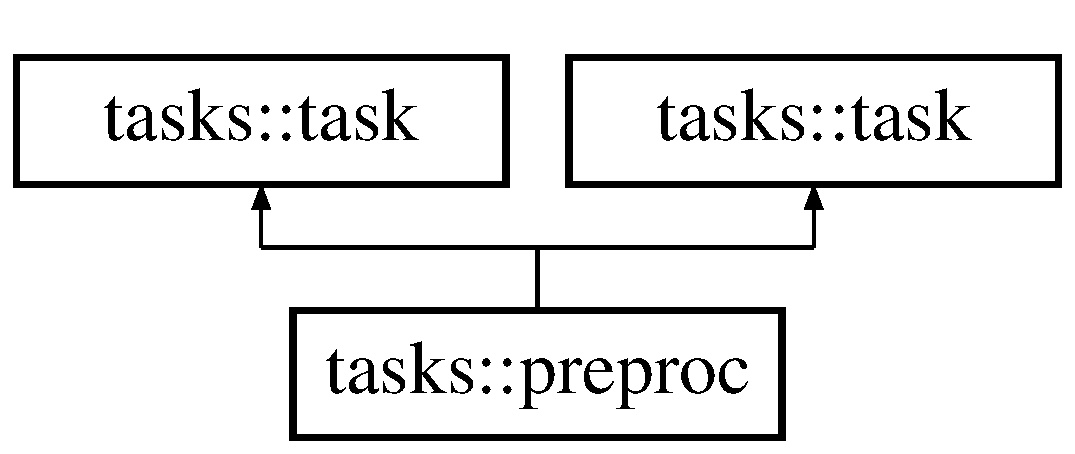
\includegraphics[height=2cm]{classtasks_1_1preproc}
\end{center}
\end{figure}
\subsection*{Public Member Functions}
\begin{CompactItemize}
\item 
def \textbf{run}\label{classtasks_1_1preproc_a151d5d52ce274050720956ef400766e}

\item 
def \textbf{run}\label{classtasks_1_1preproc_a151d5d52ce274050720956ef400766e}

\end{CompactItemize}
\subsection*{Static Public Attributes}
\begin{CompactItemize}
\item 
string \textbf{name} = '{\bfpreproc}'\label{classtasks_1_1preproc_83ad1d42b1a6909a3b46930c8fdb0aca}

\item 
string \textbf{button\-Text} = 'Preprocess frame'\label{classtasks_1_1preproc_57614188aa7924e43ca4a9adceb12d25}

\item 
string \textbf{suffix} = 'prep'\label{classtasks_1_1preproc_caee5bcb6e3ec530202af7d9bf9ebf63}

\end{CompactItemize}


\subsection{Detailed Description}


\footnotesize\begin{verbatim}Do the initial processing of the obtained frames. Includes FITS file
   verification, clipping of pre- and overscan, padding of windowed frames
   to full size and adjustment with bad pixel mask
\end{verbatim}
\normalsize
 



The documentation for this class was generated from the following files:\begin{CompactItemize}
\item 
old/PANICtool-1.0/tasks.py\item 
old/tasks.py\end{CompactItemize}
